\documentclass[../../../analisi-dei-requisiti.tex]{subfiles}

\begin{document}

\begin{figure}[H]
  \centering
  \scalegraphics{autenticazione.png}
  \caption{UUC2: Autenticazione}%
  \label{fig:uuc2}
\end{figure}

\begin{description}
  \item[Caso d’uso:] UUC2;
  \item[Titolo:] Autenticazione;
  \item[Attori primari:] utente non autenticato;
  \item[Precondizione:] il sistema deve rendere disponibile la schermata per l'autenticazione;
  \item[Postcondizione:] l'utente è autenticato al servizio;
  \item[Scenario principale:]
        \begin{enumerate}
          \item l'utente visualizza la schermata per l'autenticazione e inserisce email e password;
        \end{enumerate}
  \item[Estensioni:]
        \begin{enumerate}
          \item se la coppia email-password inserite non sono presenti all'interno del database di Stalker, allora verrà visualizzato un errore~\ref{subs:UUC2.4}.
        \end{enumerate}
\end{description}



\subsubsection{UUC2.1: Inserimento email}%
\label{subs:UUC2.1}
\begin{description}
  \item[Caso d’uso:] UUC2.1;
  \item[Titolo:] Inserimento email;
  \item[Attori primari:] utente non autenticato;
  \item[Precondizione:] il sistema deve rendere disponibile la possibilità di inserire la email per l'autenticazione;
  \item[Postcondizione:] la email inserita è corretta;
  \item[Scenario principale:]
        \begin{enumerate}
          \item l'utente inserisce la propria email per l'autenticazione;
        \end{enumerate}
  \item[Estensioni:]
        \begin{enumerate}
          \item se la email inserita non è presente nel database, si visualizzerà un errore di credenziali errate (per motivi di sicurezza non si indica qual è il campo errato)~\ref{subs:UUC2.3}.
        \end{enumerate}
\end{description}



\subsubsection{UUC2.2: Inserimento password}%
\label{subs:UUC2.2}
\begin{description}
  \item[Caso d’uso:] UUC2.2;
  \item[Titolo:] Inserimento password;
  \item[Attori primari:] utente non autenticato;
  \item[Precondizione:] il sistema deve rendere disponibile la possibilità di inserire la password per l'autenticazione;
  \item[Postcondizione:] la password inserita è corretta;
  \item[Scenario principale:]
        \begin{enumerate}
          \item l'utente inserisce la propria password.
        \end{enumerate}
  \item[Estensioni:]
        \begin{enumerate}
          \item se la password inserita non è presente nel database, si visualizzerà un errore di credenziali errate (per motivi di sicurezza non si indica qual è il campo errato)~\ref{subs:UUC2.3}.
        \end{enumerate}
\end{description}

\subsubsection{UUC2.3: Recupero credenziali}%
\label{subs:UUC2.3}

\begin{figure}[H]
  \centering
  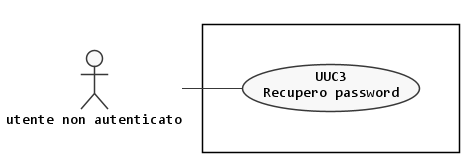
\includegraphics[width=100mm]{recupero-credenziali.png}
  \caption{UUC2.3: Recupero credenziali}%
  \label{fig:uuc2_3}
\end{figure}

\begin{description}
  \item[Caso d’uso:] UUC2.3;
  \item[Titolo:] Recupero credenziali;
  \item[Attori primari:] utente non autenticato;
  \item[Precondizione:] il sistema deve rendere disponibile la schermata di autenticazione;
  \item[Postcondizione:] l'utente si trova nella schermata di recupero credenziali;
  \item[Scenario principale:]
        \begin{enumerate}
          \item l’utente può selezionare la voce per il recupero credenziali che avviene tramite l'invio alla mail registrata di un link per reimpostare la sua password.
        \end{enumerate}
\end{description}

\subsubsection{UUC2.3.1: Recupero password}%
\label{subs:UUC2.3.1}

\begin{figure}[H]
  \centering
  \scalegraphics{recupero-password.png}
  \caption{UUC2.3.1: Recupero password}%
  \label{fig:uuc2_3_1}
\end{figure}

\begin{description}
  \item[Caso d’uso:] UUC2.3.1;
  \item[Titolo:] Recupero password;
  \item[Attori primari:] utente non autenticato;
  \item[Precondizione:] il sistema deve rendere disponibile la schermata di recupero credenziali;
  \item[Postcondizione:] l'utente ha recuperato le credenziali e può nuovamente autenticarsi;
  \item[Scenario principale:]
        \begin{enumerate}
          \item tramite questa procedura, l’utente ha la possibilità di reimpostare la password.
        \end{enumerate}
\end{description}

\subsubsection{UUC2.3.1.1: Inserimento email di registrazione}%
\label{subs:UUC2.3.1.1}
\begin{description}
  \item[Caso d’uso:] UUC2.3.1.1;
  \item[Titolo:] Inserimento email di registrazione;
  \item[Attori primari:] utente non autenticato;
  \item[Precondizione:] il sistema deve rendere disponibile la possibilità di inserire l'email di registrazione;
  \item[Postcondizione:] l'utente ha inserito correttamente la email di registrazione;
  \item[Scenario principale:]
        \begin{enumerate}
          \item l'utente si trova nella schermata per il recupero delle credenziali e inserisce l'email di registrazione.
        \end{enumerate}
  \item[Estensioni:]
        \begin{enumerate}
          \item se l'email inserita non è registrata nel database, allora verrà segnalato un errore~\ref{subs:UUC2.3.1.3}.
        \end{enumerate}
\end{description}

\subsubsection{UUC2.3.1.2: Reimpostazione password}%
\label{subs:UUC2.3.1.2}

\begin{figure}[H]
  \centering
  \scalegraphics{reimpostazione-password.png}
  \caption{UUC2.3.1.2: Reimpostazione password}%
  \label{fig:uuc2_3_1_2}
\end{figure}

\begin{description}
  \item[Caso d’uso:] UUC2.3.1.2;
  \item[Titolo:] Reimpostazione password;
  \item[Attori primari:] utente non autenticato;
  \item[Precondizione:] l'utente ha ricevuto il link presente nella email personale per reimpostare la password;
  \item[Postcondizione:] l'utente ha inserito correttamente la nuova password e ha recuperato le proprie credenziali;
  \item[Scenario principale:]
        \begin{enumerate}
          \item l'utente reimposta la password in una procedura che avviene in due passaggi:
                \begin{enumerate}
                  \item reset della vecchia password, non visibile all'utente;
                  \item inserimento della nuova password e la conferma della nuova password.
                \end{enumerate}
        \end{enumerate}
\end{description}

\subsubsection{UUC2.3.1.2.1: Inserimento nuova password}%
\label{subs:UUC2.3.1.2.1}
\begin{description}
  \item[Caso d’uso:] UUC2.3.1.2.1;
  \item[Titolo:] Inserimento nuova password;
  \item[Attori primari:] utente non autenticato;
  \item[Precondizione:] la password è resettata e l'utente inserisce la nuova password sull'apposito campo;
  \item[Postcondizione:] l'utente ha inserito correttamente la nuova password;
  \item[Scenario principale:]
        \begin{enumerate}
          \item l'utente si trova sul campo di inserimento della nuova password.
        \end{enumerate}
  \item[Estensioni:]
        \begin{enumerate}
          \item se la nuova password non rispetta determinati vincoli, verrà visualizzato un errore~\ref{subs:UUC2.3.1.2.3};
        \end{enumerate}
\end{description}

\subsubsection{UUC2.3.1.2.2: Inserimento conferma password}%
\label{subs:UUC2.3.1.2.2}
\begin{description}
  \item[Caso d’uso:] UUC2.3.1.2.2;
  \item[Titolo:] Inserimento conferma password;
  \item[Attori primari:] utente non autenticato;
  \item[Precondizione:] il sistema deve rendere disponibile la possibilità di inserire la password nuovamente per una conferma;
  \item[Postcondizione:] l'utente ha inserito correttamente la conferma della password;
  \item[Scenario principale:]
        \begin{enumerate}
          \item l'utente inserisce la password nuovamente per la conferma.
        \end{enumerate}
  \item[Estensioni:]
        \begin{enumerate}
          \item se la password inserita non è uguale a quella precedente, verrà visualizzato un errore di conferma password non valida~\ref{subs:UUC2.3.1.2.4}.
        \end{enumerate}
\end{description}

\subsubsection{UUC2.3.1.2.3: Password recupero credenziali non valida}%
\label{subs:UUC2.3.1.2.3}
\begin{description}
  \item[Caso d’uso:] UUC2.3.1.2.3;
  \item[Titolo:] Password recupero credenziali non valida;
  \item[Attori primari:] utente non autenticato;
  \item[Precondizione:] l'utente non rispetta i vincoli imposti per l'impostazione della nuova password;
  \item[Postcondizione:] l'applicazione mobile comunica all'utente l'errore;
  \item[Scenario Principale:]
        \begin{enumerate}
          \item l'utente visualizza il messaggio d'errore, in quanto la password inserita non rispetta i vincoli del sistema.
        \end{enumerate}
\end{description}

\subsubsection{UUC2.3.1.2.4: Conferma password recupero credenziali non valida}%
\label{subs:UUC2.3.1.2.4}
\begin{description}
  \item[Caso d’uso:] UUC2.3.1.2.4;
  \item[Titolo:] Conferma password recupero credenziali non valida;
  \item[Attori primari:] utente non autenticato;
  \item[Precondizione:] l'utente non inserisce correttamente la stessa password inserita nel campo precedente;
  \item[Postcondizione:] l'applicazione mobile comunica all'utente l'errore;
  \item[Scenario Principale:]
        \begin{enumerate}
          \item l'utente visualizza il messaggio d'errore, in quanto la password e la sua conferma non corrispondono.
        \end{enumerate}
\end{description}

\subsubsection{UUC2.3.1.3: Mail recupero credenziali non valida}%
\label{subs:UUC2.3.1.3}

\begin{description}
  \item[Caso d’uso:] UUC2.3.1.3;
  \item[Titolo:] Mail recupero credenziali non valida;
  \item[Attori primari:] utente non autenticato;
  \item[Precondizione:] l'utente non inserisce la mail in modo corretto;
  \item[Postcondizione:] l'applicazione mobile comunica all'utente l'errore;
  \item[Scenario Principale:]
        \begin{enumerate}
          \item l'utente visualizza il messaggio d'errore, in quanto la mail inserita non è scritta correttamente.
        \end{enumerate}
\end{description}

\subsubsection{UUC2.4: Informazioni autenticazione non valide}%
\label{subs:UUC2.4}
\begin{description}
  \item[Caso d’uso:] UUC2.4;
  \item[Titolo:] Informazioni autenticazione non valide;
  \item[Attori primari:] utente non autenticato;
  \item[Precondizione:] i dati forniti dall'utente non corrispondono a credenziali valide;
  \item[Postcondizione:] l'applicazione mobile comunica all'utente il fallimento dell'autenticazione;
  \item[Scenario principale:]
        \begin{enumerate}
          \item l'utente cerca di effettuare l'autenticazione con credenziali errate.
        \end{enumerate}
\end{description}


\end{document}
